\section{Ships, Spacelanes, and Path Finding}
\label{sec:pathfinding}

The specification made it clear --- by the way weapons and navigation between planets was to be structured --- that ship motion needed to be relatively detailed. It is no use having a weapon that can be only used in one arc if ships could instantly pivot on the spot. Instead it was desired for ships to move as large objects with a great deal of momentum, with large turning circles and ponderous movements. However it would be undesirable for the motion of ships to be too realistic, as it would make the game needlessly difficult and confusing. A real object undergoing acceleration in space could of course, accelerate essentially indefinitely (until it was nearing the speed of light) but would need to take an equal amount of time to decelerate to stop again.

\begin{marginfigure}
	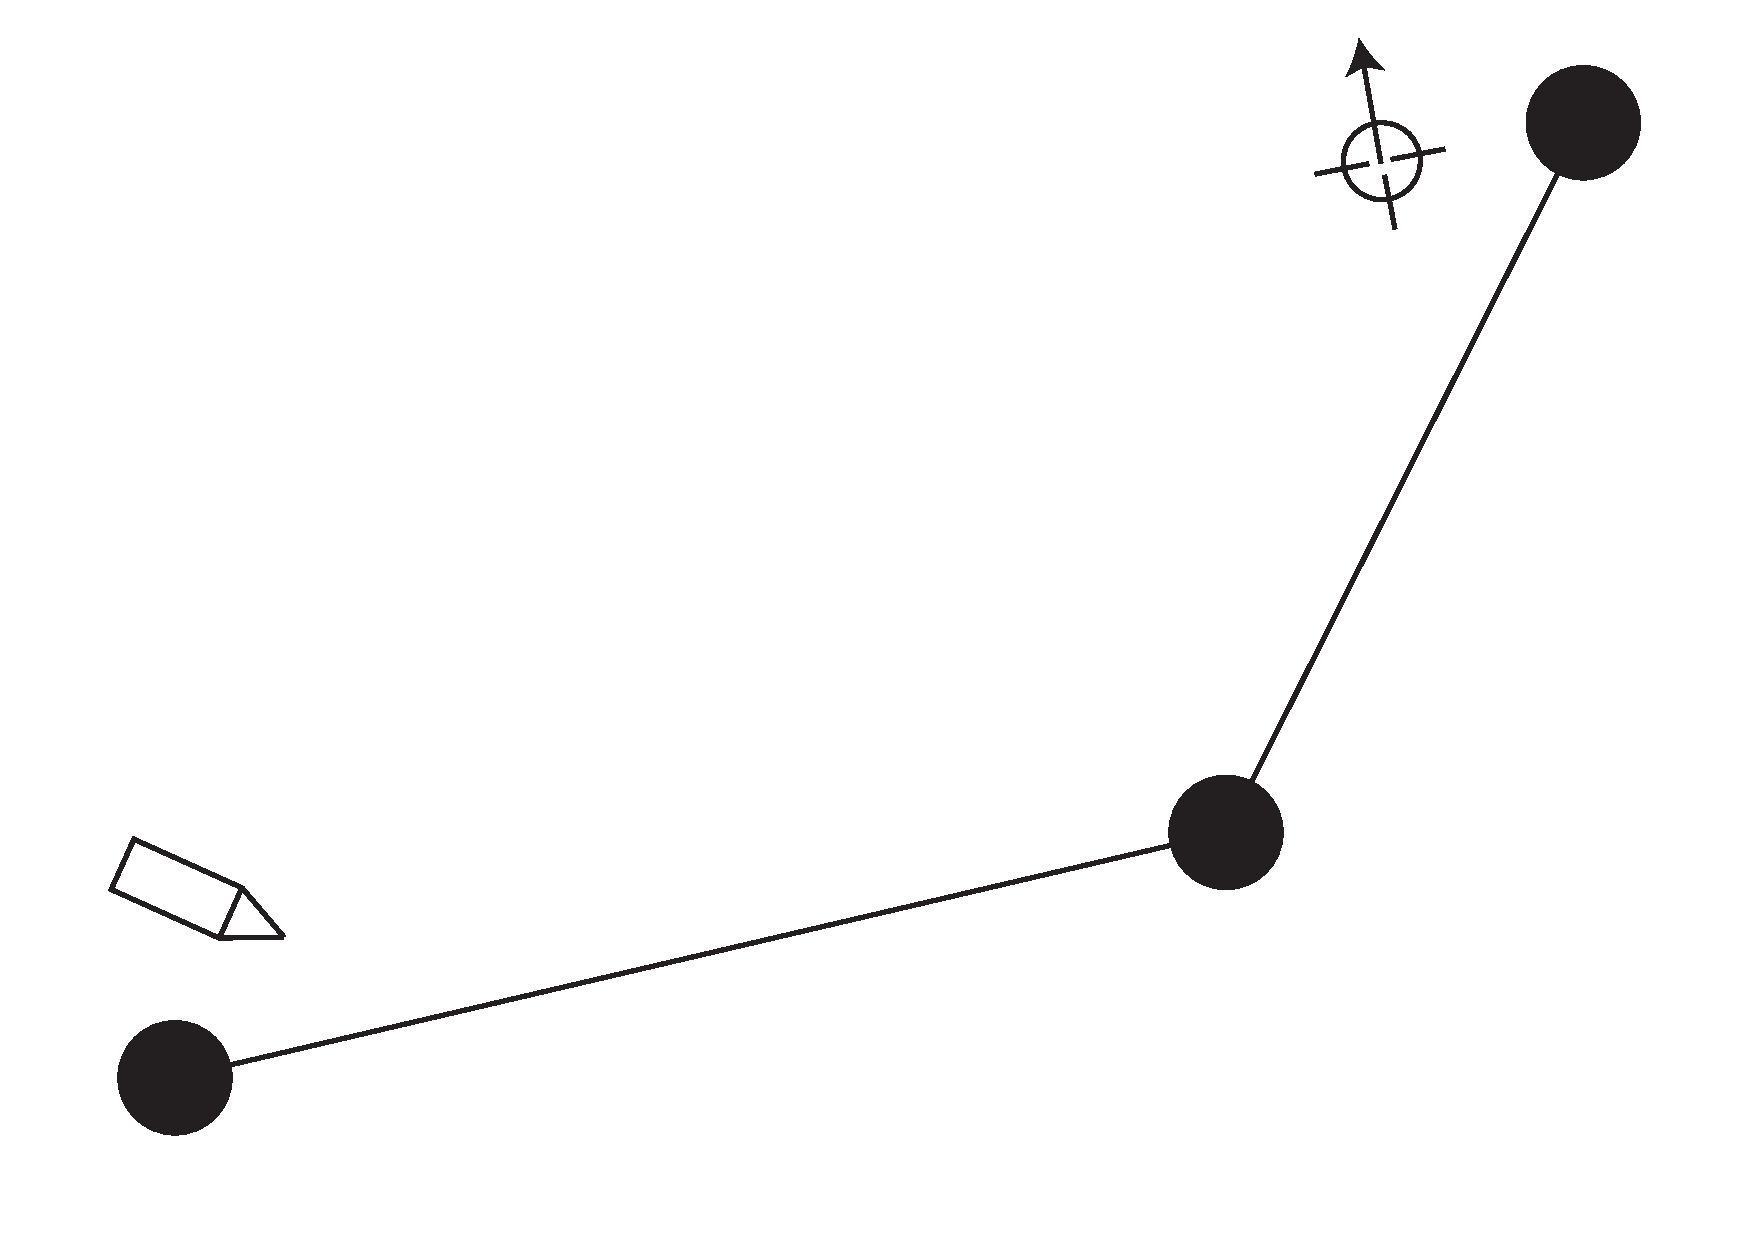
\includegraphics[width=20em]{res/pathfinding/spacelanes}
	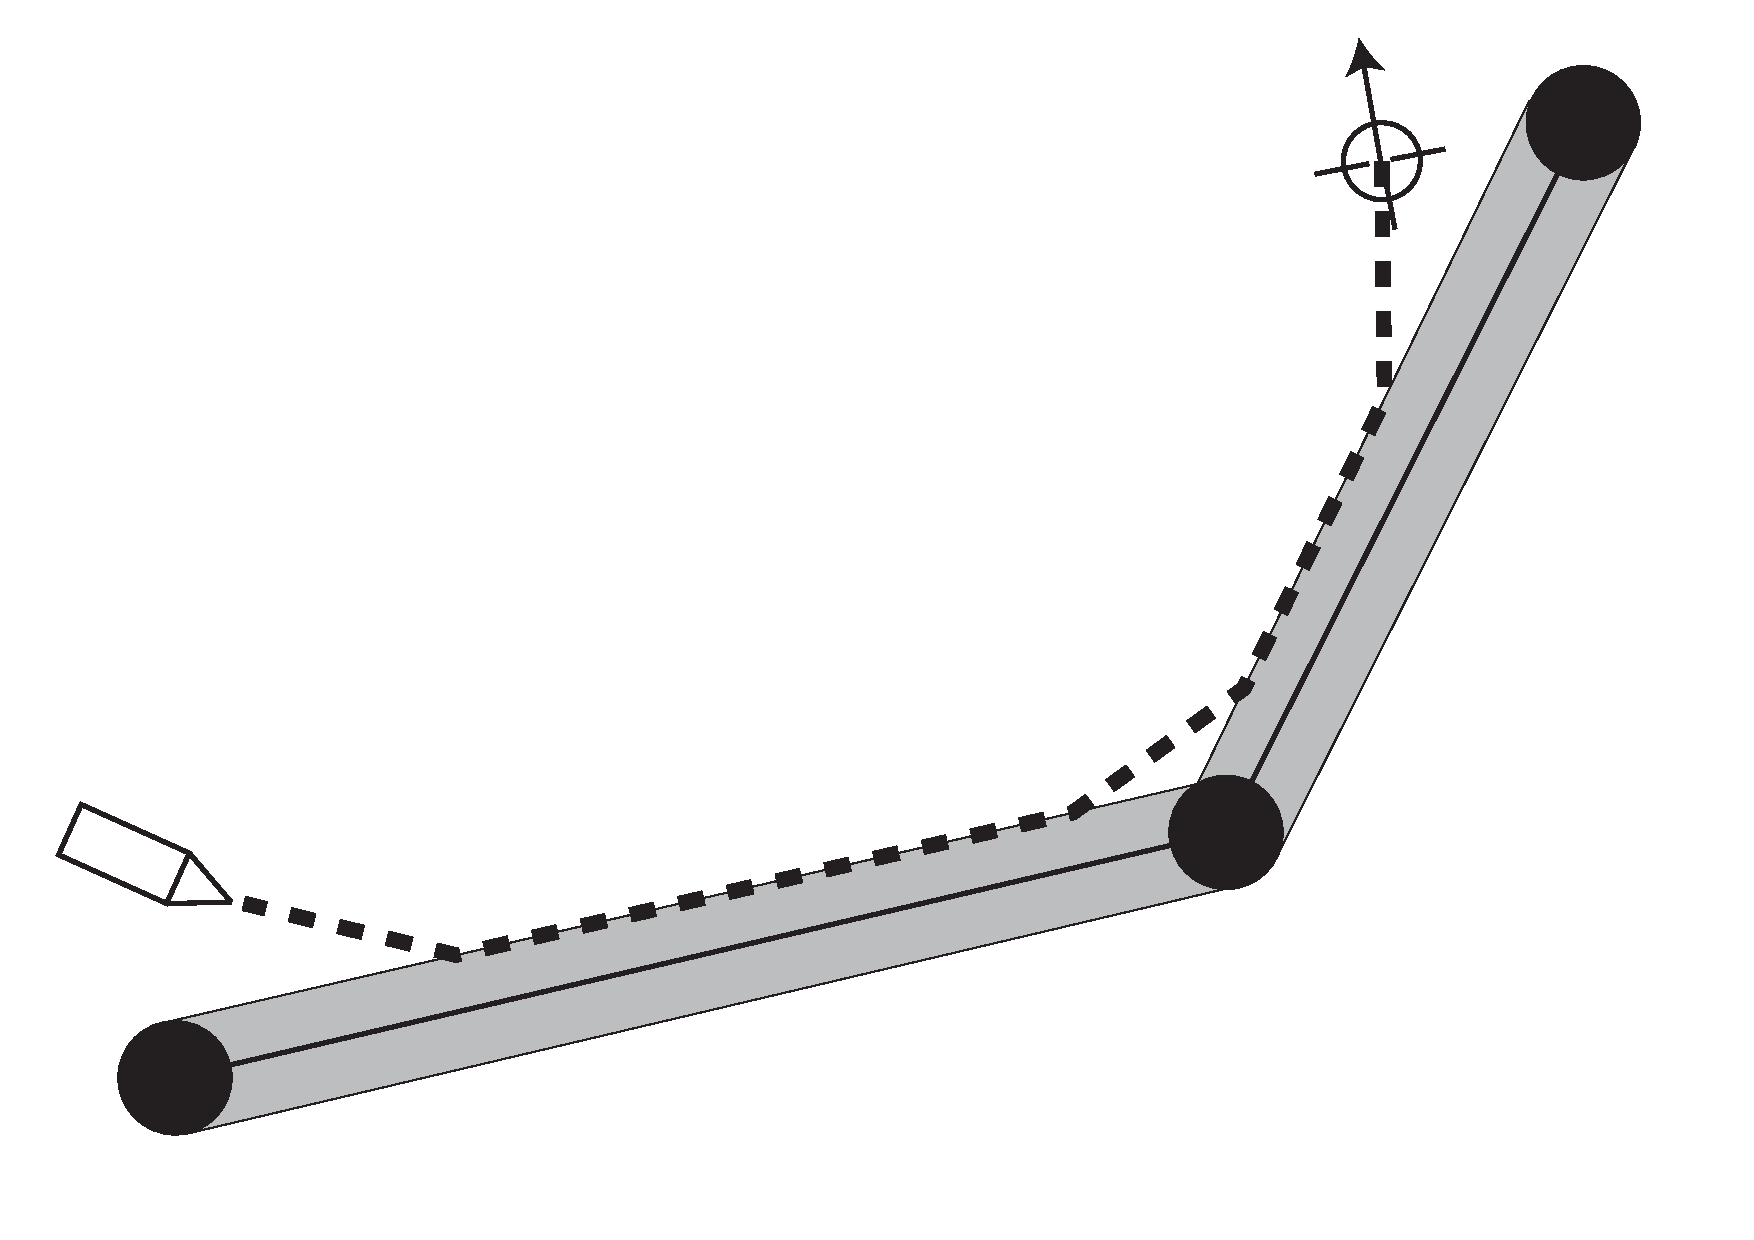
\includegraphics[width=20em]{res/pathfinding/spacelanes_ray}
	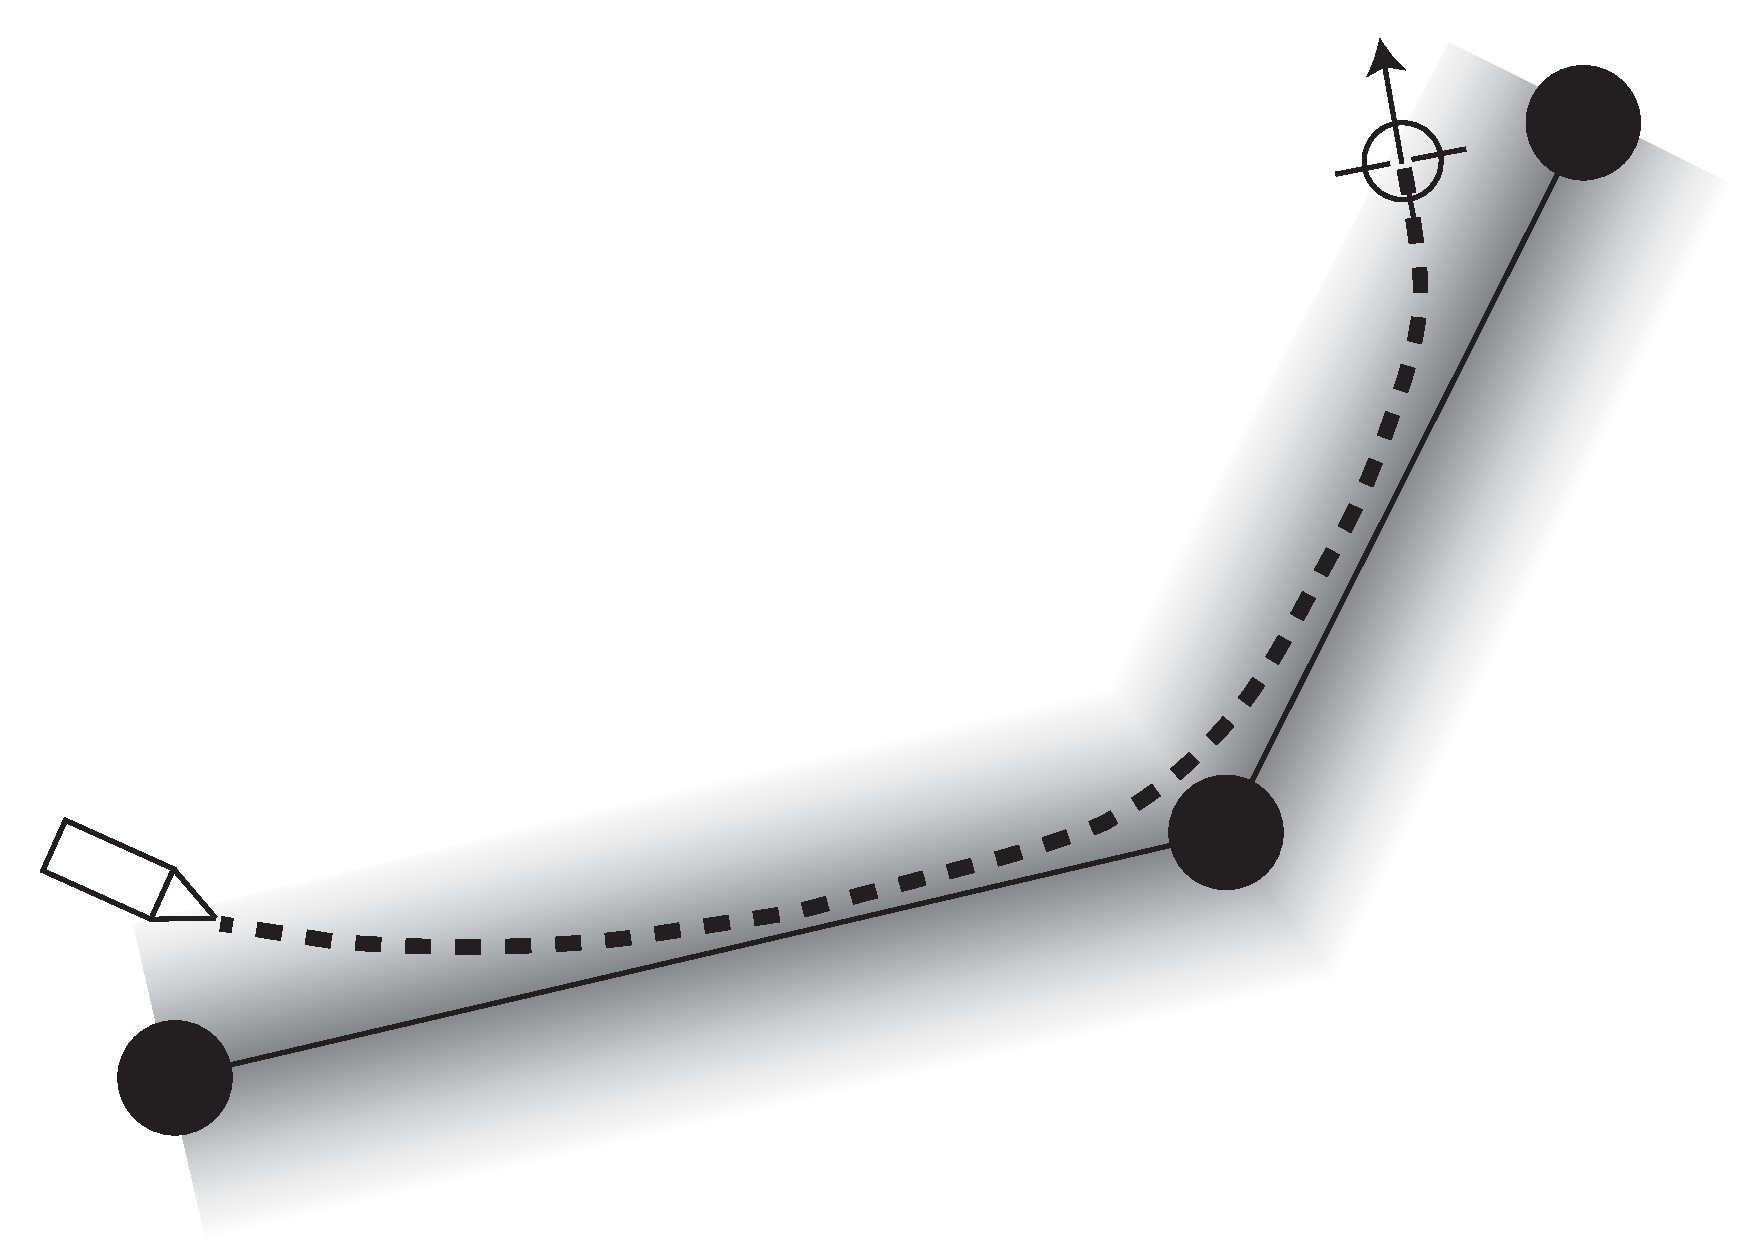
\includegraphics[width=20em]{res/pathfinding/spacelanes_field}
	\caption[Illustrations of different models for a path between current location and target utilising a spacelane.]{Illustrations of different models for a path between current location and target utilising a spacelane.}
	\label{fig:spacelanes}
\end{marginfigure}

Intimately related to these questions is the precise nature of the spacelane mechanics. Many different models were discussed for this during design meetings. Initial ideas on the physical mechanism of the spacelane was that they conferred an additional optional acceleration: i.e. that if a ship is aproximate to a lane it could opt to undergo greater acceleration than a ship far from a lane. But as mentioned, accurately modelling acceleration in space is somewhat contrary to the gameplay aspirations of the design. 

A simpler mechanics for ships that was considered to be more suitable, is for them to have a top speed that they could reach relatively quickly; but for them to still have large turning circles. This makes their motion more similar to naval ships engaged in warfare. The interpretation of the spacelane in this model cannot be simply a gain in acceleration as this confers little benefit. Instead it is clear that the spacelane must confer an addition to top speed. A possible physical interpretation of these behaviours is that the ships are moving in some kind of ether with friction, and so will reach a terminal velocity. The spacelane is then an area with an artificially induced lower density of ether.

Another fundamental question about the nature of the spacelane is whether its effects are immediately felt at full strength at a certain distance from it, or whether they fall off related to distance. the former is most definitely simpler, but the latter feels more natural as a mechanism. Figure~\ref{fig:spacelanes} shows the difference in the shortest paths that these approaches may generate, discounting the additional issue of ship turning.

\subsection{Algorithms for Pathfinding}
% physics hard
% bezier (not trivial)
% flow fields

\subsection{Applying A* to Sector}
% what is the problem
% why this is no trivial problem
% Why A*
Pathfinding for a game has 2 components: navigating a graph which represents the game, and the algorithm that traverses the graph to find the shortest route to the destination.
A* was chosen because it can guarantee an optimal solution, and it typically very fast if it has a good heuristic. 
The line of sight heuristic is typically very accurate for navigation graphs since distance between any node and the destination node is the shortest path you could get to that node.
The heuristic needs to return the time cost of getting from an arbitrary node to the destination, which is defined in Equation \ref{eq:pathfinding:cost}.
The heuristic will always assume a spacelane between the node and goal node, therefore maintaining the admissible property that it will never overestimate the cost of reaching the goal.
H big problem is that A* is designed to navigate discrete graphs, however sector is not a discrete graph.
The planets and spacelanes on the sector can be considered a discrete graph however planets are not the only locations a ship can exist at, they can move anywhere in the sector, the spacelanes just provide a speed boost.

% conversion from sector to sector graph
A solution to this problem was to generate a discrete graph from the sector graph that could then be used by A* algorithm to find a path to destination. 
In a game such as Moon Survival on page \pageref{sec:rd:moonSurvival} the world is already a discrete graph in the form of a 2-dimensional grid of squares, hence this can be traversed by the A* algorithm in-place without having to generate a separate navigation graph.

Making a discrete navigation graph that A* can traverse will require considerable memory and CPU resources depending on the number of planets and spacelanes within the sector.
An alternative to this solution would be to modify A* to traverse continuous graphs however designing a new algorithm to do this could cost considerable man hours to develop and will have no guarantees of finding a solution, let alone finding the optimal solution hence this alternative was dropped.

\begin{marginfigure}
	\includegraphics{res/pathfinding/PathFindingSector.pdf}
	\caption[Simple example of sector]{Simple example of sector with 3 planets: A, B, and C. Two points of interest are defined: P1 in the middle of the sector and P2 which is at planet A.}
	\label{fig:pathfinding:simplesector}
\end{marginfigure}

%  - example 1
To work out how to generate a navigation graph from a sector, we needed to know the ideal path the ship would take under various circumstances before being able to implement it.
In Figure \ref{fig:pathfinding:simplesector} is an example of a sector with 3 planets.
If a ship is at P2 and needs to go to planet C, it seems rather obvious: take spacelane to B then spacelane to C. 
A spacelane is faster to navigate than open space.

%  - example 2
Now consider a ship is at P1 and needs to go to planet C.
It has 3 obvious options:
\begin{itemize}
\item 
\begin{marginfigure}
	\includegraphics{res/pathfinding/PathFindingSectorOption1.pdf}
    \caption[Sector navigation - option 1: path directory to planet C]{Sector navigation - option 1: path directory to planet C.}
	\label{fig:pathfinding:simpleSectorOption1}
\end{marginfigure}
Go directly to C across open space (Figure \ref{fig:pathfinding:simpleSectorOption1})

\item 
\begin{marginfigure}
	\includegraphics{res/pathfinding/PathFindingSectorOption2.pdf}
    \caption[Sector navigation - option 2: path to B then to C]{Sector navigation - option 2: path to B then to C.}
	\label{fig:pathfinding:simpleSectorOption2}
\end{marginfigure}
Goto planet B which is close, then use it's spacelane to planet C (Figure \ref{fig:pathfinding:simpleSectorOption2})

\item 
\begin{marginfigure}
	\includegraphics{res/pathfinding/PathFindingSectorOption3.pdf}
    \caption[sector navigation - option 3: path to spacelane then to B then to C]{sector navigation - option 3: path to spacelane then to B then to C.}
	\label{fig:pathfinding:simpleSectorOption3}
\end{marginfigure}
Goto spacelane between planet A and B and use it to get to B then use it's spacelane to get to C (Figure \ref{fig:pathfinding:simpleSectorOption3}).

\end{itemize}

Traveling across open space will always be considerable slower than spacelanes so option 1 seems like a suboptimal choice, however it did bring to light the question: How fast are spacelanes?
The speed at which ships travel on spacelanes needed to be defined in order to know which route is faster.

Every ship class could have 2 properties, one defining its speed in open space and one defining its speed on spacelanes.
This method would allow the more specialisation amongst ships, allowing the concept of hit and run over spacelanes. 
It seemed logical that a slow ship on open space should be slow on a spacelane relative to a fast ship on open space, hence it seemed redundant to have 2 speed properties on a ship class.
The method chosen was to define a sector property called multiplier which specifies how much faster ships are on spacelanes relative to open space.
For example if the multiplayer was 3, then a ship with a speed of 10 in open space would have a speed of 30 on a spacelane ($ 3 \times 10 = 30 $).
This multiplayer would be applied to all ships hence it would work on the ship's base speed defined on it's ship class.
This method was simple and solved the problem.

Back to the example of considering a ship at P1 which wants to go to planet C.
If we now assume a very large value for the spacelane multiplier, then it will greatly simplify these examples, since all spacelanes will take approximately 0 seconds to use irrelevant to distance.
Under these conditions option 1 is slower then options 2 and 3.
Since P1 is closer to the spacelane between A and B it would travel across less open space then traveling to B across open space, hence option 3 is faster then option 2.

\begin{marginfigure}
	\includegraphics{res/pathfinding/PathFindingSectorOption3NavigationGraph.pdf}
    \caption[Sector navigation - option 3 navigation graph]{sector navigation - option 3 navigation graph: each circle is node on navigation graph.}
	\label{fig:pathfinding:simpleSectorOption3NavigationGraph}
\end{marginfigure}

To be able to generate a navigation graph that will allow option 3 to be a solution, the navigation graph in Figure \ref{fig:pathfinding:simpleSectorOption3NavigationGraph} would need to be generated.
In the graph there are only nodes. 
Nodes, N3, N4, and N5 were from the planets in Figure \ref{fig:pathfinding:simpleSectorOption3}.
Node N1 is the ship's starting point.
This needs to be added so the navigation graph is a connected graph.
If the destination wasn't a planet then a node would need to be added for this as well, but since the destination is a planet, no new node needs adding.

Node N2 doesn't correspond to any planet, start point or destination point, it corresponds to where the ship needs to enter the spacelane.
It is a node that has no corresponding point on the original sector, it is a virtual node added to allow an optimal path to the solution.

The optimal solution is now: $N1 \to N2 \to N3 \to N4$.

For A* to make the same conclusion, costs needed to be associated with each edge on the navigation graph in Figure \ref{fig:pathfinding:simpleSectorOption3NavigationGraph}.
Since we want to minimise the time to destination, it makes sense to use "time to traverse an edge" metric.
To calculate this metric, the following equation is used:
$$ time = \frac{distance}{speed} $$
The distance can easily be calculated using Pythagorean theorem, and the speed is simply the ship class's speed.
This works for open space edges but what about spacelanes? Obviously this will be much faster.
To make the formula work for both open space and spacelanes the multiplayer needed to be factored in, giving the following formula:
\begin{equation} \label{eq:pathfinding:cost}
\frac{distance}{speed \times multiplier}
\end{equation}

In open space the $multiplier$ is 1.0, and on spacelanes it is whatever the sector defines it as.

To generate a navigation graph from a sector the following needs adding to the navigation graph:
\begin{itemize}
\item node for each planet in the sector
\item edge between all planet nodes where a spacelane was
\item a node for start location unless it is a planet
\item a node for destination location unless it is a planet
\end{itemize}

We also need to make it a fully connected graph, i.e. from any planet you can get to any other planet.
This is true within the sector no matter where you are on the sector you can get to any other point in a strait line. 
The only reason other points may be added to the path is for speed.

The node N2 in Figure \ref{fig:pathfinding:simpleSectorOption3NavigationGraph} still has not been added.
The question "how do we define where to add nodes on spacelanes and how many to add" is not soo simple to answer.
Two example sectors were used to answer that question, the examples are shown in Figure \ref{fig:pathfinding:sectorExample2} and \ref{fig:pathfinding:sectorExample3}.

\begin{marginfigure}
	\includegraphics{res/pathfinding/PathFindingSector2.pdf}
    \caption[Sector example 2: cross-over edges]{Sector example 2: cross-over edges.}
	\label{fig:pathfinding:sectorExample2}
\end{marginfigure}
In Figure \ref{fig:pathfinding:sectorExample2} the ship starts at P1 and it's destination is P2.
To get there it should take the spacelane $C \to D$ up to point N1 then switch over to spacelane $A \to B$.
For A* to find this path it would require adding a virtual node at the intersection of spacelanes.

\begin{marginfigure}
	\includegraphics{res/pathfinding/PathFindingSector3.pdf}
    \caption[Sector example 3: right-angle]{Sector example 3: right-angle.}
	\label{fig:pathfinding:sectorExample3}
\end{marginfigure}
In Figure \ref{fig:pathfinding:sectorExample3} both the start point P1 and the destination point P2 are in open space.
The optimal solution is outlined in dotted lines.
The lines from A to B and C to B are spacelanes.
For A* to find the optimal path outlined it would require virtual nodes N1 and N2.
Finding where to put these optimal nodes in the navigation graph is the hard part.
In this example a simple case could be:
\begin{itemize}
\item if start point is in open space add virtual node at closest point on closest spacelane
\item if destination point is in open space add virtual node at closest point on closest spacelane
\end{itemize}
This would add the virtual nodes N1 and N2 in this example.

\begin{marginfigure}
	\includegraphics{res/pathfinding/PathFindingSector4.pdf}
    \caption[Sector example 4: closest spacelane is not your friend]{Sector example 4: closest spacelane is not your friend.}
	\label{fig:pathfinding:sectorExample4}
\end{marginfigure}

Example in Figure \ref{fig:pathfinding:sectorExample4} breaks the previous rule.
Before it is explained why it breaks the rule, it is assumed that the multiplier is a relatively low value, such that it is quicker to get to the destination P2 by traveling directly to P2 across open space rather than to N1.
The rule is broken because the start point P1 is in open space and the closest point on the closest spacelane, N1 is not the used in the optimal solution.
Hence a virtual edge between P1 and P2 is also added, this fixes the problem.
It also allows navigation on sectors without any planets.

There were many corner cases where a new virtual edge would be needed besides the examples provided.
Instead of having many corner case rules for adding virtual nodes on spacelanes, there was a brute force solution where virtual nodes are added at regular intervals on every spacelane. 
This will result in the possibility of a virtual node not existing at the optimal location on an edge but there will be one close to the optimal position.
Though this solution is is not an optimal solution it is close and guarantees a path will be found, which provided enough benefits over the other options to pick this one.

% problems this method causes (not optimal solution but close)
There is no requirement that the path be optimal, it is purely a preference hence as long as the path is reasonable, the pathfinding will be considered a success, hence the brute force solution was chosen.
Performance is a large issue with the brute-force method of generating a graph, because it adds an exponential number of nodes and edges compared to the original sector. 

% navigation of sector graph
Once the discrete navigation graph was generated from the sector, it could be given to the A* algorithm which would generate the optimal path around the sector.


